\documentclass[../../main.tex]{subfiles}

\begin{document}
\graphicspath{{img/}{02_theory/img/}}

\chapter{Lý thuyết tính toán song song trên nền tảng CUDA}

\section{CUDA là gì?}
CUDA (Compute Unified Device Architecture) là kiến trúc phần cứng và phần mềm phục vụ việc tính toán trên GPU. CUDA được phát triển bởi NVIDIA vào năm 2007.

GPU giúp thực hiện một số lượng lớn các nhiệm vụ đồng thời và nhanh chóng bằng cách sử dụng nhiều ALU. Trước khi có CUDA, các ALU được lập trình thông qua các API đồ họa. Hình \ref{fig:gpu_vs_cpu} mô tả cấu thúc GPU so với CPU. Sử dụng CUDA giúp điều khiển GPU mà không cần tham chiếu các API đồ họa. 

CUDA phù hợp với các thuật toán có khả năng được thực hiện song song và các dataset lớn.

\begin{figure}[H]
    \begin{center}
        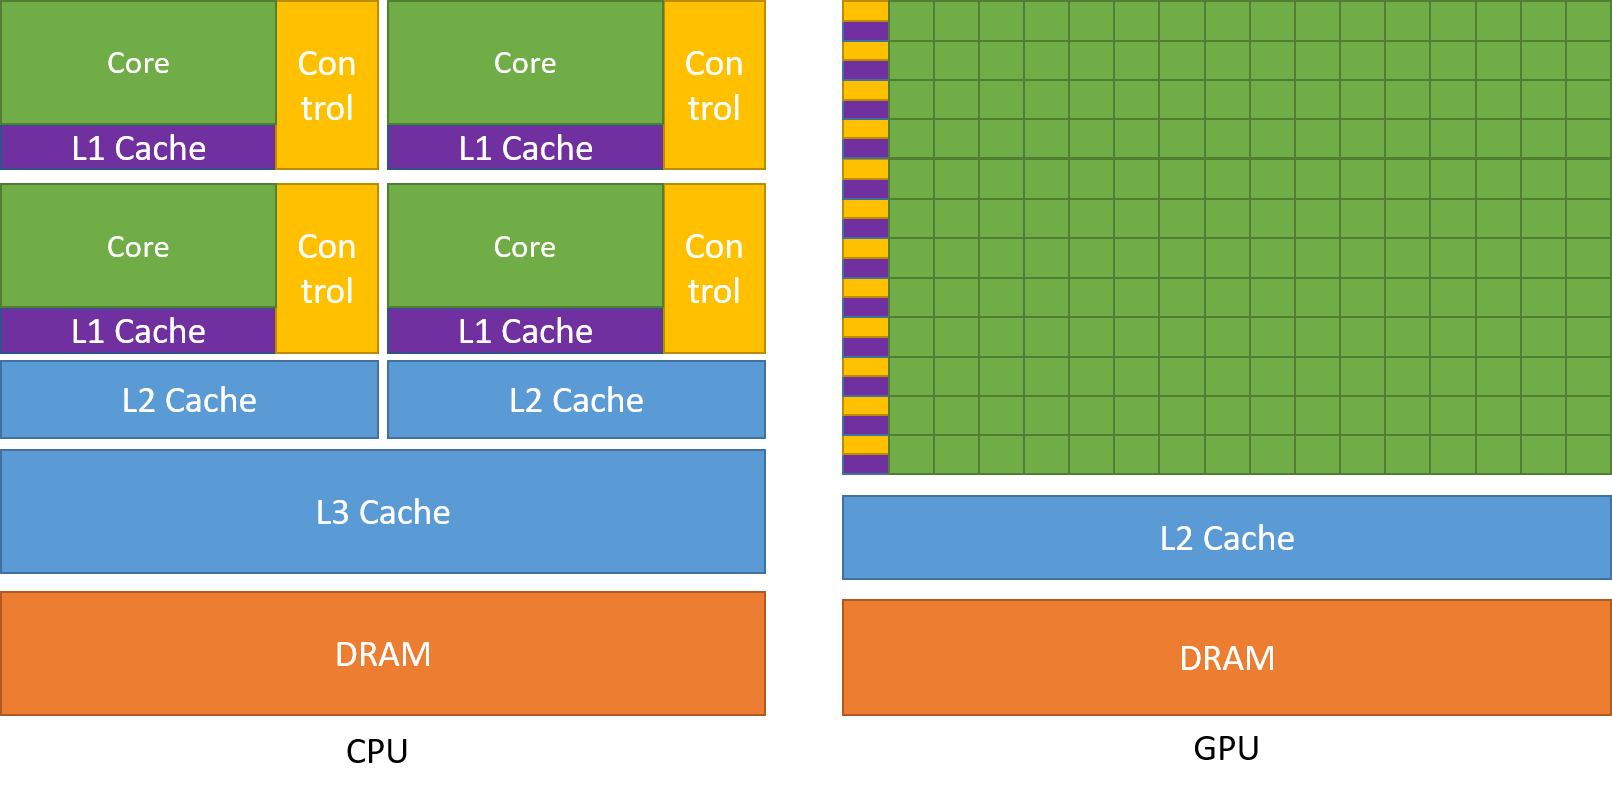
\includegraphics[scale=0.5]{gpu-devotes-more-transistors-to-data-processing.png}
    \end{center}
    \caption{Kiến trúc GPU và CPU}
    \label{fig:gpu_vs_cpu}
\end{figure}

\section{CUDA kernel và CUDA thread}
Ta định nghĩa một số khái niệm chung như sau:
\begin{itemize}
    \item Device: là GPU, nơi thực hiện phần tính toán song song của ứng dụng.
    \item Host: là CPU, nơi thực hiện phần tính toán nối tiếp của ứng dụng.
    \item Kernel: là hàm chạy trên device.
\end{itemize}
Host và device thường được kết nối thông qua các cổng PCI.

\subsection*{Thread}
Một CUDA kernel sẽ được thực thi bằng một mảng các thread. Tất cả các thread đó sẽ chạy cùng một code. Tuy nhiên, mỗi thread sẽ có một ID riêng để tính toán địa chỉ vùng nhớ mà thread đó sẽ xử lý. Hình \ref{fig:cuda-thread} mô tả tổng quan cách một kernel được thực thi. Từ hình ta thấy các thread từ 0 đến 7 chạy cùng một chương trình, chương trình sẽ lấy dữ liệu dựa vào threadID, xử  lý và cuối cùng xuất dữ liệu ra vào một vị trí cũng được tính toán dựa trên threadID.

\begin{figure}[H]
    \begin{center}
        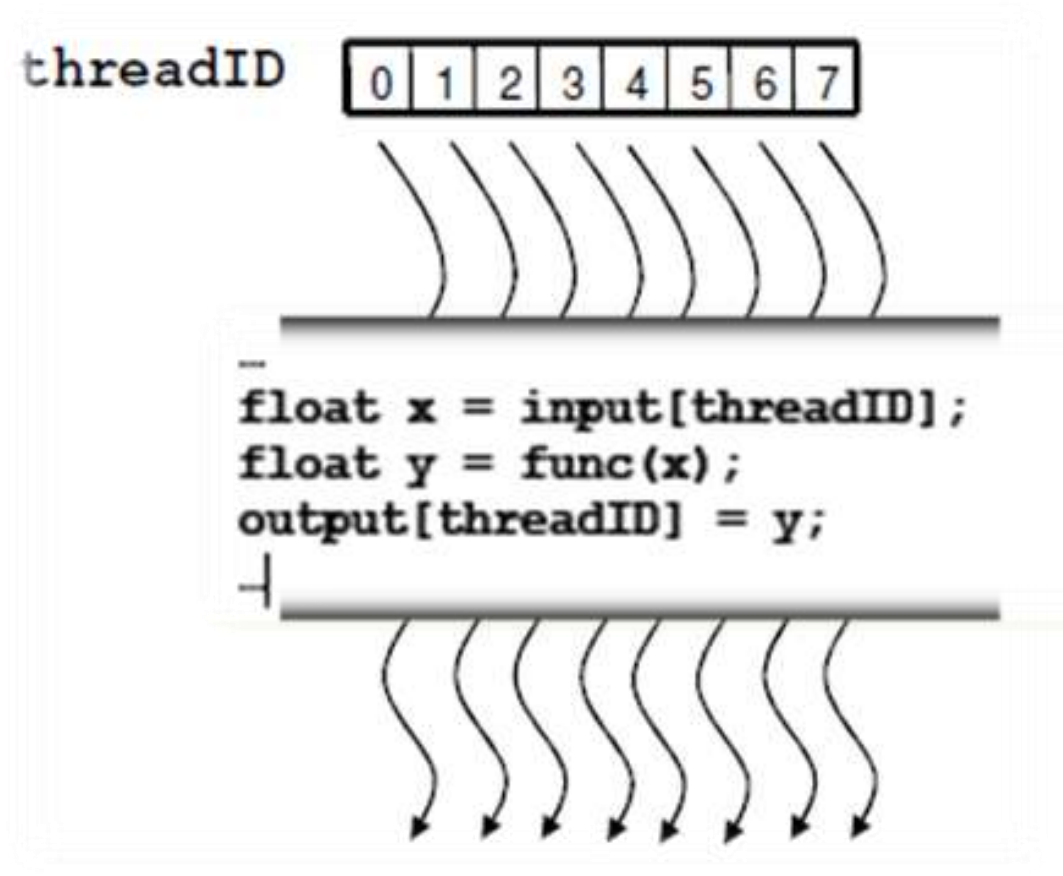
\includegraphics[scale=0.2]{cuda-thread.png}
    \end{center}
    \caption{CUDA Thread}
    \label{fig:cuda-thread}
\end{figure}

\subsection*{Block và grid}
Một tập các thread có thể kết hợp để hoàn thành một nhiệm vụ tạo thành một block. Các block được phân biệt bằng blockID. Một tập các block tạo thành grid. 
Hình \ref{fig:cuda-structure} mô tả cấu trúc này của CUDA.
\begin{figure}[H]
    \begin{center}
        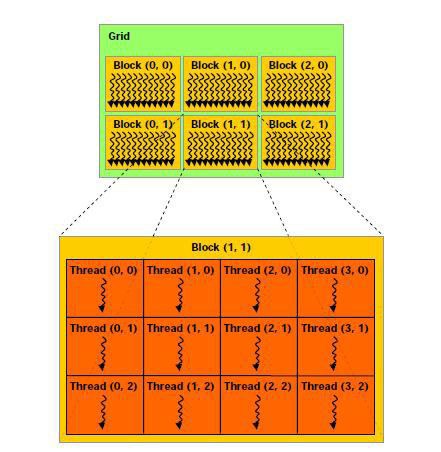
\includegraphics[scale=0.6]{CUDA-Grid-Block-Thread-Structure-1-2.png}
    \end{center}
    \caption{Cấu trúc CUDA}
    \label{fig:cuda-structure}
\end{figure}

\section{CUDA Memory Model}
Vì kernel là một chương trình được thực thi độc lập bởi các thread nên mỗi thread sẽ cần những thanh ghi (registers) và một vùng nhớ riêng (local memory). Các thread trong cùng một block có thể chia sẻ chung một vùng nhớ gọi là shared memory. Các block trong grid lại chia sẻ một số vùng nhớ chung lớn hơn bao gồm global memory, constant memory và texture memory.
\begin{figure}[H]
    \begin{center}
        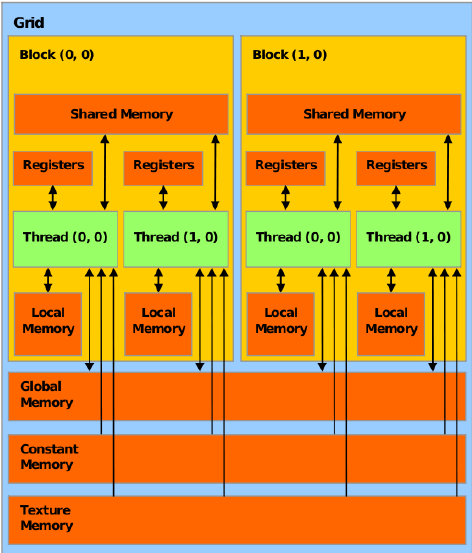
\includegraphics[scale=0.5]{CUDA-memory-model-from-7.png}
    \end{center}
    \caption{CUDA Memory Model}
    \label{fig:CUDA Memory Model}
\end{figure}

\section{Thư viện CUDA}
NVDIA hỗ trợ săn nhiều bộ thư viện giúp việc lập trình trở ên dễ  thuận tiện hơn:
\begin{itemize}
    \item cuBLAS: thư viện hỗ  trợ các phép toán đại số tuyến tính
    \item cuFFT: thư viện Fast Fourier Transform
    \item nvJPEG: Hỗ  trợ xử lý ảnh JPEG
    \item cuRAND: Hỗ trợ tạo số ngẫu nhiên
\end{itemize}
Chương trình có sử dụng CUDA cần được compile bằng nvcc compiler của NVIDIA.

\section{Lập trình song song trên nền tảng CUDA}
Cấu trúc một chương trình có sử dụng CUDA khá tương tự một chương trình viết bằng C/C++. Chương trình có sử dụng CUDA sẽ bắt đầu bằng phần chương trình chạy trên CPU như các ứng dụng thông thường. Tại các vị trí cần tính toán song song, chương trình chạy trên CPU sẽ gọi các kernel theo cú pháp riêng của CUDA để các hàm đó được chạy song song trên GPU. Hình \ref{fig:cuda-example} mô tả một chương trình đơn giản thực hiện việc tính toán cộng hai vector bằng CUDA.

\begin{figure}[H]
\begin{lstlisting}[language=C++,
    basicstyle=\footnotesize\ttfamily,
    numbers=left,
    numberstyle=\footnotesize,
    tabsize=2,
    breaklines=true,
    escapeinside={@}{@},
    numberstyle=\tiny\color{solarized@base01},
    keywordstyle=\color{solarized@green},
    stringstyle=\color{solarized@cyan}\ttfamily,
    identifierstyle=\color{solarized@blue},
    commentstyle=\color{solarized@base01},
    emphstyle=\color{solarized@red},
    frame=single,
    rulecolor=\color{solarized@base2},
    rulesepcolor=\color{solarized@base2},
    showstringspaces=false]
// Kernel definition
__global__ void VecAdd(const float* A, const float* B, float* C, int N) {
    int tid = blockDim.x * blockIdx.x + threadIdx.x;
    if (tid < N) C[tid] = A[tid] + B[tid];
}
        
void main() {
    float *h_A, *h_B, *h_C; // host copies of a, b, c
    float *d_A, *d_B, *d_C; // device copies of a, b, c
    int size = N * sizeof(float);

    // Alloc space for device copies of a, b, c
    cudaMalloc((void**)&d_A, size);
    cudaMalloc((void**)&d_B, size);
    cudaMalloc((void**)&d_C, size);

    // Alloc space for host copies of a, b, c and setup input values
    h_A = (int*)malloc(size); random_ints(h_A, N);
    h_B = (int*)malloc(size); random_ints(h_B, N);
    h_C = (int*)malloc(size); 

    // Copy inputs to device
    cudaMemcpy(d_A, h_A, size, cudaMemcpyHostToDevice);
    cudaMemcpy(d_B, h_B, size, cudaMemcpyHostToDevice);

    // Launch VecAdd() kernel on GPU
    int numBlocks= (N + 255)/256;
    int threadPerBlock = 256;
    VecAdd<<<numBlocks, threadPerBlock>>>(d_A, d_B, d_C, N); // Note the <<<blocksPerGrid, 256>>>

    // Copy result back to host
    cudaMemcpy(h_C, d_C, size, cudaMemcpyDeviceToHost);

    // Cleanup
    free(h_A); free(h_B); free(h_C);
    cudaFree(d_A); cudaFree(d_B); cudaFree(d_C); 
}
\end{lstlisting}
\caption{Ví dụ CUDA}
\label{fig:cuda-example}
\end{figure}

Ở dòng 2, từ khóa $\_\_global\_\_$ được dùng để chỉ rằng hàm này được gọi từ CPU và thực thi trên GPU. 

Dòng 13,14,15, malloc một số vùng nhớ trên RAM của GPU các thread sử  dụng. 

Dòng 18,19,20 khởi tạo dữ liệu trên RAM của CPU. 

Dòng 23,24 copy dữ liệu từ RAM của CPU lên RAM của GPU. 

Ở dòng 29, kernel được gọi, ngoài các tham số  như được khai báo ở dòng 2, ta cần truyền vào số lượng block ($numBlocks$) và số lượng thread ($threadPerBlock$) sẽ thực hiện kernel. Sau khi gọi hàm, $numBlocks \times threadPerBlock$ thread sẽ cùng chạy kernel. ID của thread được tính bằng công thức:
\begin{equation}
tid = blockDim.x * blockIdx.x + threadIdx.x
\end{equation}
Trong đó:
\begin{itemize}
    \item $blockDim.x$: số lượng thread trong 1 block, luộn bằng tham số $threadPerBlock$ đã được truyền vào khi gọi hàm.
    \item $blockIdx.x$: ID của block.
    \item $threadIdx.x$: ID của thread trong block $blockIdx.x$
\end{itemize}

\end{document}